\documentclass{standalone}
\usepackage{tikz}

\begin{document}

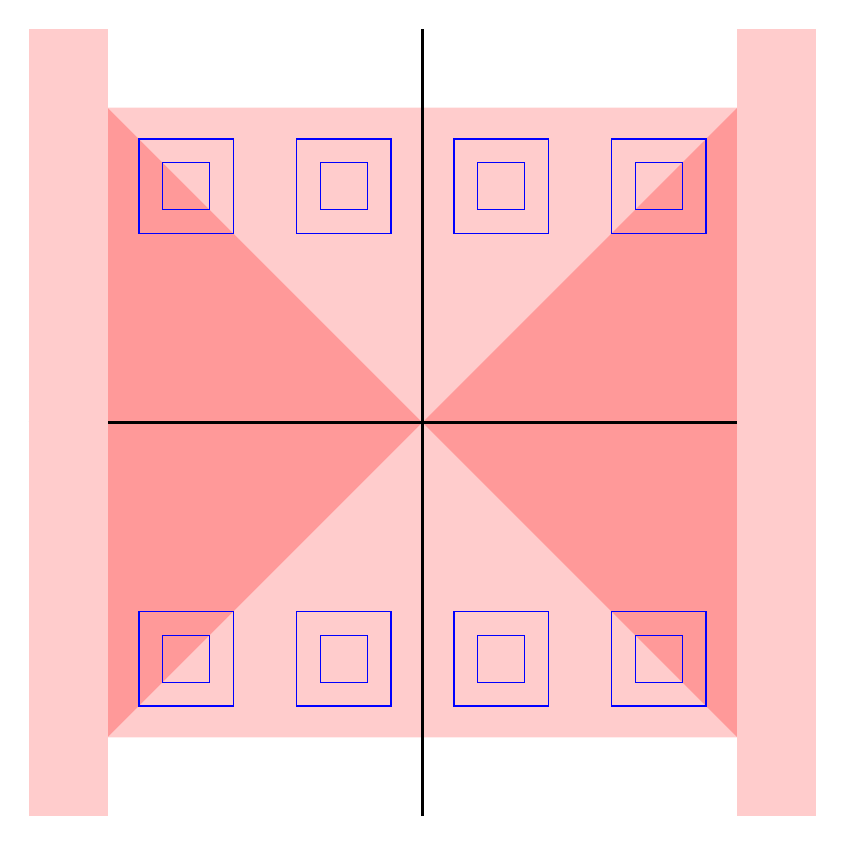
\begin{tikzpicture}
    % Colors
    \fill[red!20] (-4,-4) -- (0,0) -- (4,-4) -- cycle;
    \fill[red!20] (-4,4) -- (0,0) -- (4,4) -- cycle;
    \fill[red!40] (-4,-4) -- (0,0) -- (-4,4) -- cycle;
    \fill[red!40] (4,-4) -- (0,0) -- (4,4) -- cycle;
    
    % Axis lines
    \draw[thick] (-5,0) -- (5,0);
    \draw[thick] (0,-5) -- (0,5);
    
    % Blue rectangles
    \foreach \x in {-3,-1,1,3} {
        \foreach \y in {-3,3} {
            \draw[blue] (\x-0.3,\y-0.3) rectangle (\x+0.3,\y+0.3);
            \draw[blue] (\x-0.6,\y-0.6) rectangle (\x+0.6,\y+0.6);
        }
    }
    
    % Red shaded areas near y-axis
    \fill[red!20] (-5,0) rectangle (-4,5);
    \fill[red!20] (-5,0) rectangle (-4,-5);
    \fill[red!20] (4,0) rectangle (5,5);
    \fill[red!20] (4,0) rectangle (5,-5);
    
\end{tikzpicture}

\end{document}